% NYU Fall 2026 Deep Learning, Project 1 report.
% Built on the AAAI Press LaTeX template linked by the course
% (https://www.overleaf.com/latex/templates/aaai-press-latex-template/jymjdgdpdmxp):
% Style provenance is documented in STYLE_SOURCE.md.
% The template forbids hyperref, natbib, geometry, titlesec, caption and T1 fontenc; none is used here.
\documentclass[letterpaper]{article}
\usepackage{aaai}
\nocopyright
\ifdefined\XeTeXversion
\usepackage[OT1]{fontenc}
\fi
\usepackage{times}
\usepackage{helvet}
\usepackage{courier}
\usepackage{url}
\usepackage{graphicx}
\usepackage{booktabs}
\usepackage{amsmath}
\frenchspacing
\ifdefined\pdfinfo
\setlength{\pdfpagewidth}{8.5in}
\setlength{\pdfpageheight}{11in}
\pdfinfo{
/Title (A 4.8M-Parameter Residual Network for CIFAR-10 under a Parameter Budget)
/Author (Jiaqi Li)}
\else
\setlength{\paperwidth}{8.5in}
\setlength{\paperheight}{11in}
\special{pdf:docinfo << /Title (A 4.8M-Parameter Residual Network for CIFAR-10 under a Parameter Budget) /Author (Jiaqi Li) >>}
\fi
\setcounter{secnumdepth}{2}

\title{A 4.8M-Parameter Residual Network for CIFAR-10 under a Parameter Budget}
\author{Jiaqi Li\\
New York University, CS-GY 6953 / ECE-GY 7123 Deep Learning, Fall 2026\\
Kaggle team: \texttt{jiaqi li nyu}\\
% The repository is private during the competition; make it public before submitting this report.
Code: \url{https://github.com/Songard/cifar-10-res-net-architecture-challenge-dl}
}

\begin{document}
\maketitle

\begin{abstract}
We design and train from scratch a residual convolutional network for 10-class CIFAR-10 image classification
under a budget of 5 million trainable parameters. Our final network keeps the full-width first three stages of
ResNet-18 and trims the parameter-heavy last stage to a single 352-channel block, for 4,797,002 parameters and
453M multiply-accumulates per image. We pair it with a stronger training recipe: TrivialAugment, Cutout, label
smoothing, a weight moving average, flip test-time augmentation and bf16 mixed precision. At the same 100-epoch
budget, the new architecture and recipe together raise held-out validation accuracy from 94.48\% (a
2.8M-parameter half-width ResNet-18 with the baseline recipe) to 96.42\%; we did not separate the two
contributions. On the 1,000-image public half of the competition's hidden test set, the same model scores
86.30\%. We attribute the 10-point gap to a likely distribution shift between the training and test images.
Without test labels this remains a hypothesis, and we discuss what our evidence can and cannot rule out.
\end{abstract}

\section{Overview}
The task is to classify $32\times32$ RGB images into ten classes with a convolutional network that has skip
connections and at most 5,000,000 trainable parameters, trained from scratch on the 50,000 official training
images. No pretrained weights or external data are allowed. Kaggle scores predictions on 2,000 hidden test
images drawn from ``a version of'' CIFAR-10 \cite{krizhevsky2009learning}. These are split 50/50 into a public
leaderboard, visible during the competition, and a private leaderboard that decides the final ranking.

Our findings in brief:
\begin{itemize}
\item \textbf{Compute per parameter is cheap in the right places.} Most of ResNet-18's 11.2M parameters sit in its
last stage, which runs at $4\times4$ resolution. Trimming only that stage keeps 82\% of ResNet-18's compute within
our budget. On the Apple GPU we trained on, the final network ran at 0.72$\times$ the throughput of a uniformly
narrowed ResNet-18 with 1.9$\times$ its multiply-accumulates.
\item \textbf{Strong regularization changes the training dynamics.} With the improved recipe, training accuracy
on augmented batches ends at only 87.7\% even though the model is larger, while held-out accuracy reaches
96.0--96.4\%. The baseline, by contrast, fits its training batches almost perfectly (99.9\%) and stops at 94.5\%.
\item \textbf{Held-out validation overstates hidden-test accuracy here.} The validation split is drawn from the
training distribution; the hidden test set appears not to be.
\end{itemize}

\section{Data and Evaluation Protocol}
We split the 50,000 labeled images once, stratified by class with seed 2026, into 45,000 training and 5,000
validation images (500 per class). We checked that no pixel-identical image crosses the split. Per-channel
normalization statistics are computed on the 45,000 training images only. Every model selection decision below
uses this fixed validation split. The hidden test images are used only to write the submission file; their
labels are unavailable to us, and we never adapt to the test images, for example by re-estimating
batch-normalization statistics or pseudo-labeling.

Validation accuracy on 5,000 images has a standard error of about 0.27 percentage points at 96\% accuracy. The
1,000-image public leaderboard has a standard error of about 1.1 points at 86\%, so small public-score
differences are not meaningful.

\section{Methodology}
\subsection{Residual architecture}
Every network we considered is built from the residual block described in the assignment,
\begin{equation}
y = \mathrm{ReLU}\big(S(x) + \mathrm{BN}(\mathrm{conv}(\mathrm{ReLU}(\mathrm{BN}(\mathrm{conv}(x)))))\big),
\end{equation}
with $3\times3$ convolutions, where $S$ is the identity, or a $1\times1$ convolution with batch normalization
\cite{ioffe2015batch} when the resolution or width changes \cite{he2016deep}. A $3\times3$ stem replaces the
ImageNet $7\times7$ stem and max-pool, following the CIFAR adaptation in the instructor-recommended
reference code \cite{kuangliu}. Each network ends with global average pooling and one linear layer.
Table~\ref{tab:archs} lists the candidates.

\begin{table}[t]
\centering
\footnotesize
\setlength{\tabcolsep}{3.6pt}
\begin{tabular}{@{}lccrr@{}}
\toprule
Name & Widths & Blocks & Params & MACs \\
\midrule
ResNet-18 (reference) & 64--512 & 2,2,2,2 & 11.17M & 555M \\
\texttt{resnet18-w32} (baseline) & 32--256 & 2,2,2,2 & 2.80M & 139M \\
\texttt{resnet18-w42} & 42--336 & 2,2,2,2 & 4.82M & 240M \\
\texttt{resnet18-64-352} (final) & 64--352 & 2,2,2,1 & 4.80M & 453M \\
\texttt{resnet20-x4} & 64--256 & 3,3,3 & 4.33M & 648M \\
\bottomrule
\end{tabular}
\caption{Candidate residual networks: stage widths, residual blocks per stage, trainable parameters and
multiply-accumulates (MACs) per $32\times32$ image. All parameters are counted, including batch normalization and
the classifier.}
\label{tab:archs}
\end{table}

\paragraph{Design rationale.} In ResNet-18 the fourth stage holds most of the parameters but only a small share of
the compute, because it runs on $4\times4$ feature maps. Shrinking every stage uniformly to fit the budget
(\texttt{resnet18-w42}) also shrinks the high-resolution stages, which do most of the computation. Our final
network, \texttt{resnet18-64-352}, keeps stages 1--3 of ResNet-18 at full width (64, 128 and 256 channels at
$32\times32$, $16\times16$ and $8\times8$). Stage 4 becomes one 352-channel block. The parameters break down as:
stem 1,856; stage 1 147,968; stage 2 525,568; stage 3 2,099,712; stage 4 2,018,368; classifier 3,530; total
\textbf{4,797,002}. This leaves a 4\% margin under the limit while keeping 82\% of ResNet-18's MACs. We also
defined a deeper three-stage alternative in the style of ResNet-20 and wide ResNets
\cite{he2016deep,zagoruyko2016wide}, \texttt{resnet20-x4}; its 100-epoch run was paused after 35 epochs
(Section~Results).

\subsection{Training recipes}
Both recipes use SGD with Nesterov momentum 0.9, weight decay $5\times10^{-4}$, cross-entropy, a linear warmup over
5 epochs followed by cosine decay \cite{loshchilov2017sgdr}, and the same split and seed (Table~\ref{tab:recipes}).

\begin{table}[t]
\centering
\small
\begin{tabular}{@{}lll@{}}
\toprule
Setting & Baseline & Improved \\
\midrule
Batch size, peak LR & 128, 0.1 & 256, 0.2 \\
LR updates & per epoch & per step \\
Weight decay on BN/bias & yes & no \\
Crop padding & zeros, 4 px & reflect, 4 px \\
Policy augmentation & none & TrivialAugmentWide \\
Cutout & none & $16\times16$ \\
Label smoothing & 0 & 0.1 \\
Weight EMA (per step) & none & 0.999 \\
Test-time augmentation & none & horizontal flip \\
Precision & fp32 & bf16 autocast \\
\bottomrule
\end{tabular}
\caption{Training recipes. Both use random crops and horizontal flips, 100 epochs and seed 2026.}
\label{tab:recipes}
\end{table}

The improved recipe adds standard regularizers for small-image classification:
\begin{itemize}
\item TrivialAugmentWide \cite{muller2021trivialaugment}, which applies one randomly chosen image operation at a
random strength;
\item Cutout \cite{devries2017improved}, which erases a random square after normalization;
\item label smoothing \cite{szegedy2016rethinking};
\item an exponential moving average (decay 0.999) of the weights and batch-normalization statistics, an
exponentially weighted variant of iterate averaging \cite{polyak1992acceleration}, used for evaluation;
\item averaging the logits of each image and its mirror image at test time.
\end{itemize}
Weight decay is restricted to convolution and linear weights. The batch size and learning rate double together.

\subsection{Implementation}
We trained on an Apple M5 Pro laptop (20-core GPU, 48~GB unified memory) with PyTorch 2.15 on the Metal (MPS)
backend. Random crops, flips and Cutout run batched on the GPU; TrivialAugment runs per image in six CPU
data-loader workers. Mixed precision \cite{micikevicius2018mixed} with bfloat16 autocast keeps weights and
optimizer state in fp32. Each run records its full configuration, source-file hashes and per-epoch metrics, and
saves checkpoints with model, EMA, optimizer and random-number-generator states, so training can resume from any
epoch; the 100-epoch baseline continued from its 5-epoch pilot checkpoint. A test suite covers the parameter
budget, augmentation geometry, the learning-rate schedule, EMA, test-time augmentation, split isolation and the
submission writer. We do not claim bitwise determinism across devices.

\section{Results}
\subsection{Held-out validation}
Table~\ref{tab:results} compares the two runs, which differ in both architecture and recipe, at the same
100-epoch budget; Figure~\ref{fig:curves} shows the curves. The improved model reaches 96.02\% with EMA weights and
96.42\% with flip test-time augmentation, 1.94 points above the baseline's 94.48\%. Selecting the best epoch on the
validation set instead of the last would give a slightly optimistic 94.60\% for the baseline; we report last-epoch
values throughout.

\begin{table}[t]
\centering
\small
\begin{tabular}{@{}lcccc@{}}
\toprule
Run (100 epochs) & Params & Raw & EMA & EMA+flip \\
\midrule
Baseline & 2.80M & 94.48 & -- & -- \\
Improved & 4.80M & 95.90 & 96.02 & \textbf{96.42} \\
\bottomrule
\end{tabular}
\caption{Last-epoch accuracy (\%) on the 5,000 held-out validation images.}
\label{tab:results}
\end{table}

\begin{figure*}[t]
\centering
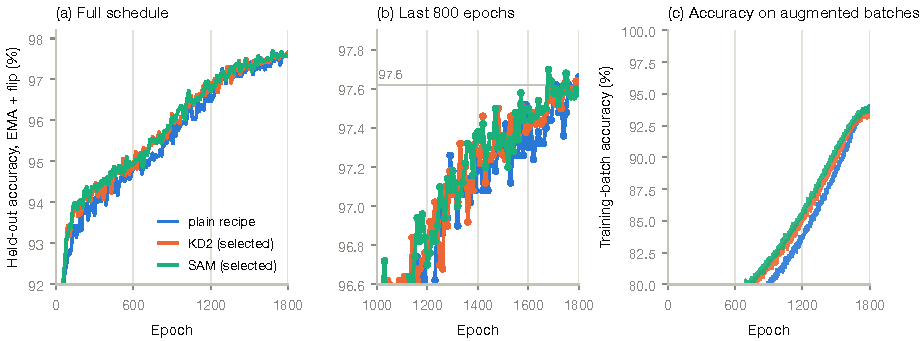
\includegraphics[width=0.82\textwidth]{figures/curves.pdf}
\caption{Left: held-out validation accuracy. EMA weights lead the raw weights while the learning rate is high.
Right: accuracy on augmented training batches. The improved recipe leaves a large gap between training and
validation accuracy, a sign of strong regularization rather than overfitting.}
\label{fig:curves}
\end{figure*}

\paragraph{Architecture at matched epochs (partial).} With the improved recipe and the same seed,
\texttt{resnet20-x4} reached 91.38\% EMA validation accuracy at epoch 35 of 100 (85.46\% raw), against 91.08\%
(85.30\%) for \texttt{resnet18-64-352} at the same epoch. The run was then paused. The difference is within the
sampling error of the validation set for a single seed, and mid-schedule accuracy need not predict the final
ranking, so we draw no conclusion between the two architectures.

\paragraph{Where the gains come from.} The improvement is broad: every class improves
(Figure~\ref{fig:perclass}). The largest gain is for cat (87.8\% to 92.8\%), the hardest class. Cat and dog
confusions still dominate the remaining errors (21 cats predicted as dog and 20 dogs as cat out of 500 each),
followed by birds predicted as airplanes or cats.

\begin{figure*}[t]
\centering
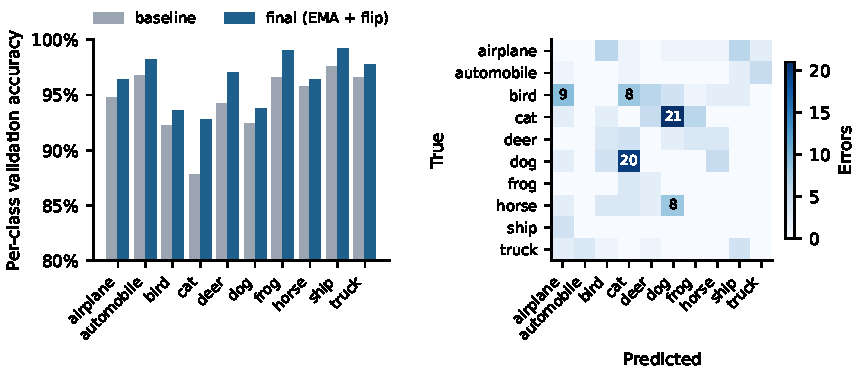
\includegraphics[width=0.82\textwidth]{figures/per_class.pdf}
\caption{Left: per-class held-out accuracy of the baseline and of the final model (EMA weights, flip TTA). Right:
off-diagonal confusion counts of the final model; cells with at least 8 errors are labeled.}
\label{fig:perclass}
\end{figure*}

\subsection{Cost}
Wall-clock training time was 0.29~h for the baseline and 0.54~h for the improved run. The improved run trains at
about 2,575 images/s, compared with 4,531 for the fp32 baseline at batch 128. Process memory stayed below 0.8~GB
in both runs; sampled GPU driver allocation peaked at 3.4~GB. A short benchmark (Figure~\ref{fig:speed}) shows
bf16 autocast running 1.6--2.4$\times$ faster than fp32 on this GPU, and the final network at 0.72$\times$ the
throughput of \texttt{resnet18-w42} despite 1.9$\times$ its compute, which made the full-width early stages
affordable.

\begin{figure}[t]
\centering
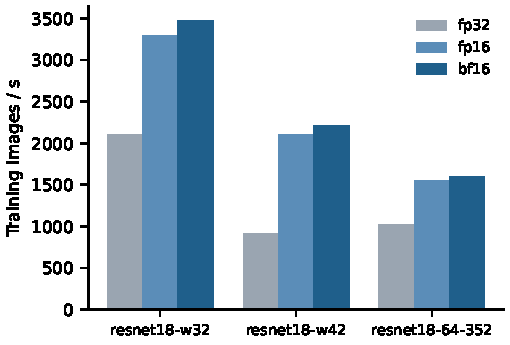
\includegraphics[width=\columnwidth]{figures/speed.pdf}
\caption{Training throughput at batch 256 by precision (20-step benchmark, synchronized every step, with its own
data loading; absolute values are below full-epoch throughput, so compare bars only relative to each other).}
\label{fig:speed}
\end{figure}

\subsection{Hidden test set}
We submitted the improved model's predictions (EMA weights, flip test-time augmentation). Kaggle reports a
\textbf{public test accuracy of 86.30\%}; the private score is released after the competition closes. At
submission time this ranked 7th on the public leaderboard, where the leading entry had 89.20\%.

The roughly 10-point gap between validation (96.42\%) and public test accuracy (86.30\%) is far larger than
sampling error. Our validation images are a random subset of the official training distribution, while the test
images come from ``a version of'' CIFAR-10. A careful reproduction of the CIFAR-10 test set produced accuracy drops
of 3--15 percentage points across a broad range of models \cite{recht2019imagenet}, and every public leaderboard
entry was below 90\% at the time. We therefore treat validation accuracy as a ranking signal, not an estimate of
test accuracy, and keep selecting models on held-out validation rather than on leaderboard feedback.

\section{Discussion}
\paragraph{Architectural trade-offs.} Uniform narrowing is simple and keeps the ResNet-18 layout, but it gives up
compute exactly where small images need it. Trimming only the last stage keeps the high-resolution stages intact at
the cost of a much thinner final representation (one block instead of two). Deeper three-stage designs such as
\texttt{resnet20-x4} add even more compute per parameter (648M vs.\ 453M MACs). On the MPS backend, theoretical
MACs were a poor predictor of training time: \texttt{resnet18-64-352} ran at 0.72$\times$ the throughput of
\texttt{resnet18-w42} with 1.9$\times$ its MACs. We did not run a controlled test of why, for example of channel
alignment or kernel sizes, and did not benchmark \texttt{resnet20-x4} in isolation.

\paragraph{Lessons learned.} (1) The 5-epoch pilot (77.6\%) said little about the final accuracy; full schedules
were needed before comparing anything. (2) Strong augmentation lowers training accuracy sharply. That is expected,
and EMA weights recover much of the noise of the raw weights during training. (3) Per-step learning-rate updates
exposed a bug: an epoch-level warmup formula overshot the peak rate by 20\% when evaluated mid-epoch. We fixed it
and reran from scratch. (4) Independently re-reading every submission file before upload caught a crash in the
prediction audit for newer checkpoints before it could affect a submission.

\paragraph{Limitations.} The comparison in Table~\ref{tab:results} changes the architecture and the recipe at
the same time. A recipe-only ablation (the improved recipe on \texttt{resnet18-w32}) was planned but not run, and
the \texttt{resnet20-x4} run was paused after 35 of 100 epochs, so we do not attribute the gain between
architecture and recipe. All numbers come from a single seed. The public score is based on 1,000 images and a
single submission. We cannot verify the cause of the validation--test gap without test labels, so distribution
shift is our hypothesis rather than a finding. Two checks argue against, but do not rule out, a test-pipeline
error: the predicted class counts are close to uniform (178--214 per class out of 2,000), and test images are
normalized with the same training-set statistics as the validation images. A 200-epoch run of the final recipe on
all 50,000 images was started but paused after 41 epochs; it has no held-out data, so we report no result from it.
Longer and full-data training usually improves accuracy further.

\section{Conclusion}
A residual network that keeps ResNet-18's high-resolution stages and trims its last stage fits the 5M-parameter
budget at 4,797,002 parameters. Trained from scratch with standard modern regularization, it reaches 96.42\%
held-out validation accuracy and 86.30\% public test accuracy on the competition's hidden set. Next steps are
longer full-data training, running the controlled ablations, and teacher--student distillation from our own
from-scratch models.

% TODO for the author: add any AI-assistance statement the course requires, in your own words.

\bibliographystyle{aaai}
\bibliography{references}

\end{document}
